% !TeX spellcheck = it_IT



\section{Cosa sono i Bitcoin?}

Bitcoin è una valuta elettronica creata nel 2008 da Satoshi Nakamoto, uno pseudonimo dietro al quale non si sa ancora con la precisione chi si nasconde.
Con il termine Bitcoin viene denotata sia la rete che consente il possesso e il trasferimento di denaro, sia la moneta. Per convenzione, Bitcoin si riferisce alla tecnologia della rete, mentre \textit{bitcoin} alla valuta stessa.

Come ogni valuta, i bitcoin possono essere trasferiti tramite gli utenti, grazie ad un protocollo che viene rispettato all'interno della rete Internet, il quale può essere eseguito su differenti dispositivi, in modo tale da permettere la fruibilità del servizio anche attraverso gli smartphones.
 
I bitcoins possono essere comprati, venduti e scambiati con altre valute, tramite degli organismi specializzati nel cambio di monete virtuali. In un certo senso, Bitcoin è la forma perfetta di denaro per Internet, dal momento che è estremamente veloce, sicuro e senza limiti.

A differenza delle altre valute, i bitcoin sono esclusivamente virtuali, dietro di essi non esistono monete fisiche. Tali bitcoin vengono coinvolti in transazioni da mittente a ricevente, i quali possiedono delle chiavi crittografiche pubbliche e private che servono per trasmettere e sbloccare la spesa dei bitcoin ricevuti.
Infatti, senza la chiave privata, chi riceve i bitcoin non può spenderli in nessun modo. Tali chiavi vengono conservate all'interno di un \textit{wallet}, letteralmente un "portafoglio". Ogni wallet è caratterizzato da un indirizzo Bitcoin il quale è univoco e ha la funzione di fare riferimento ad uno dei partecipanti alla transazione. In questo modo, quando viene effettuato uno scambio di bitcoin, vengono visualizzati solamente gli indirizzi dei wallet. Questa caratteristica permette quindi di rendere anonime le transazioni, dato che agli indirizzi non è connesso in nessun modo il nome o il cognome dell'individuo o dell'associazione che interviene nello scambio.

La rete Bitcoin, oltre ad essere completamente virtuale, è priva di un'unità centralizzata, infatti essa è costituita da un sistema distribuito peer-to-peer.\\
I bitcoin vengono creati tramite un processo, detto \textit{mining}, che permette a chiunque di mettersi in competizione per trovare una soluzione ad un problema matematico. Ogni persona che partecipa alla rete bitcoin, potrebbe operare come un \textit{miner}, ovvero colui che cerca di risolvere il problema matematico per generare bitcoin, usando le capacità del proprio computer messo a disposizione della computazione.\\

Quando viene effettuato uno scambio di bitcoin tra due o più wallet, viene creata una \textit{transazione}. Ogni transazione viene conservata in una struttura dati chiamata \textbf{blocco}, il quale a sua volta va a costituire la \textbf{Blockchain}.

\subsection{Bitcoin: Panoramica}

Nella \textit{figura\ref{fig:overview}}, si può notare che il sistema bitcoin comprende: utenti con wallet che contengono chiavi, transazioni che sono propagate attraverso la rete, e miner che forniscono (attraverso una computazione competitiva) il consenso alla blockchain, la quale è il libro mastro di tutte le transazioni.

In questo paragrafo si andrà a tracciare il percorso di una singola transazione quando viene propagata attraverso la rete, e le interazioni tra ogni componente del sistema, ad alto livello.

\begin{figure}[h]
	\centering
	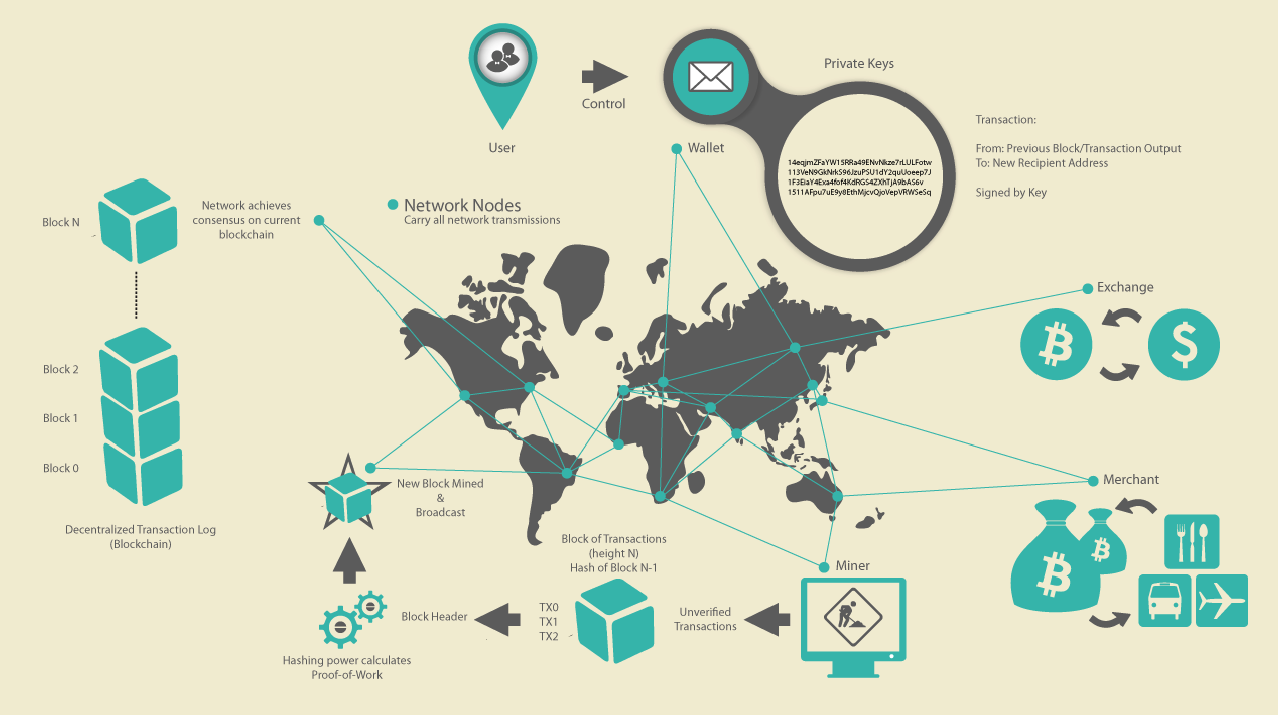
\includegraphics[width= \linewidth]{figure/overview}
	\caption{\textit{Bitcoin overview} \label{fig:overview}}
\end{figure}


\section{Cos'è la Blockchain?}
La Blockchain, letteralmente \textit{catena di blocchi}, è una base di dati distribuita, che permette la memorizzazione delle transazioni raggruppate in blocchi connessi tra loro, ognuno con il suo successivo. Ogni blocco è una struttura dati che contiene un numero variabile di transazioni, inserite dal \textit{miner} che ha minato il blocco, fino ad un tetto massimo di 1MB per singolo blocco.\\

L'idea di base della Blockchain, deriva dal concetto di \textbf{libro mastro}, il registro della contabilità in cui sono riuniti tutti i conti che compongono un dato sistema contabile. In questo caso il sistema contabile sarebbe la rete Bitcoin, mentre la Blockchain sarebbe il libro mastro che contiene tutti i conti, ovvero le transazioni. \\

L'antico libro mastro, veniva utilizzato come fonte ufficiale per la memorizzazione degli scambi e dei passaggi di proprietà. Infatti, quando veniva fatta una compravendita tra mittente e ricevente, veniva controllato sul libro mastro se il ricevente non avesse speso precedentemente il denaro, e se il mittente non avesse già venduto la merce usata nello scambio.

Infine, se fosse andato tutto a buon fine, veniva registrata la transazione sul libro mastro, in modo da essere consultabile e pubblica per le successive transazioni.

Un principio importante di questo meccanismo è la fiducia, la quale tutti ripongono nel libro mastro: ognuno si fida del gestore della memorizzazione delle transazioni, al punto che, chi compra e chi vende, può effettuare scambi anche senza fidarsi reciprocamente. Quindi, il libro mastro è una garanzia, sia per il mittente che per il ricevente dello scambio. Inoltre, le banche possono perciò controllare gli scambi che vengono fatti e il denaro posseduto da ogni partecipante alle transazioni.

La Blockchain, come già sottolineato, è una struttura dati composta da diverse unità di base, dette blocchi. Infatti, blockchain significa letteralmente \textit{catena di blocchi}.

Quindi, tali blocchi vengono "incatenati", ovvero collegati tra loro tramite un protocollo ben definito nella struttura del sistema bitcoin. 

Ogni blocco all'interno della blockchain, è identificato da un codice hash, generato applicando l'algoritmo di crittografia SHA256 all'header del blocco. Un singolo blocco è collegato al suo predecessore, conosciuto come "blocco genitore", attraverso il campo \textit{previous block hash} all'interno del proprio header. In altre parole, ogni blocco contiene l'hash del proprio blocco genitore all'interno dell'header. Infine, la sequenza dei vari hash genera una catena che collega tutti i blocchi all'indietro, fino al blocco numero zero.

\subsection{Mining}

Le monete bitcoin sono "coniate" durante la creazione di ciascun blocco ad un tasso fisso. Ogni blocco, generato all'incirca ogni 10 minuti, contiene nuovi bitcoin, creati da zero.
Il \textit{mining} inoltre serve per proteggere il sistema bitcoin contro transazioni fraudolente o transazioni che cercano di spendere gli stessi bitcoin più di una volta, problema conosciuto con il nome di \textit{double-spend} (doppia-spesa).

I miner validano le transazioni e le registrano sul \textit{ledger} globale, ovvero la Blockchain, creando un nuovo blocco e inserendo le transazioni al suo interno, per poi aggiungere il blocco alla chain (=catena). Perciò, i miner raccolgono un certo numero di transazioni e cercano di inserirle all'interno di un nuovo blocco creato appositamente. Tutte le transazioni che poi risultano alla fine all'interno di tale blocco, sono considerate \textit{confirmed} (=confermate), ovvero una sorta di etichetta che permette al ricevente di tali bitcoin di spenderli successivamente.

Lo scopo dei miner è quello di guadagnare bitcoin, e possono ottenerli in due modi: 
\begin{itemize}
	\item quando un nuovo blocco viene aggiunto alla Blockchain, si ottiene un premio in bitcoin
	\item per ogni transazione vengono pagate le \textit{fees} (=tasse) al miner
\end{itemize}

Al fine di ottenere il premio, i miner devono trovare la soluzione ad un problema matematico molto difficile basato su un algoritmo di crittografia. La soluzione a tale problema, chiamata \textbf{proof of work}, è inclusa all'interno del nuovo blocco, e serve come prova che il miner ha impiegato un notevole sforzo di elaborazione. La competizione tra i miner per trovare la proof of work per guadagnare bitcoin è alla base della sicurezza del sistema Bitcoin.

Il processo della generazione di nuove monete è chiamato \textbf{mining} perchè la ricompensa è progettata in modo da simulare rendimenti decrescenti, esattamente come l'estrazione di metallo prezioso.
La fornitura di valuta bitcoin è creata attraverso il mining, analogamente alla procedura con cui una banca centrale crea moneta stampando banconote. 

L'ammontare del premio del mining a Gennaio 2009 era di 50 bitcoin per blocco e a Novembre 2012 già si era dimezzato fino ad ottenere 25 bitcoin. Attualmente il guadagno del premio del mining risulta 12.5 bitcoin per blocco.
Seguendo questo processo, il premio per il mining di un blocco, decrescerà esponenzialmente fino all'anno 2140, quando tutti i bitcoin (20.9999998 milioni) saranno emessi. All'incirca dopo il 2140 non saranno più prodotti nuovi bitcoin e il miner andrà a guadagnare solamente tramite le tasse applicate per ogni transazione.

I miners guadagnano bitcoin per ogni transazione tramite le tasse. Esse vengono calcolate come eccesso di bitcoin tra le transazioni di input e quelle di output. Infatti, il miner che riesce a creare il nuovo blocco "tiene il resto" di ogni transazione inclusa in quel blocco. \\ Dopo il 2140, tutti i bitcoin potranno essere guadagnati tramite tasse.

La parola "mining", ovvero minare, potrebbe avere un significato ingannevole poichè sembrerebbe indicare l'estrazione di metallo prezioso, e quindi focalizza l'attenzione sul premio che viene ottenuto dal minatore.\\
Sebbene il mining sia incentivato dal suo guadagno, il suo obiettivo principale non è il premio in denaro o la creazione di nuove monete.\\ 
Mining è il processo principale per la decentralizzazione del sistema, nel quale le transazioni sono validate e chiare. Rappresenta una sicurezza per il sistema e permette lo sviluppo di una rete basata sul consenso, senza l'intervento di un'autorità centrale.

\subsection{Consenso Decentralizzato}

La Blockchain non essendo creata da un'autorità centrale, è assemblata indipendentemente da ogni nodo all'interno della rete. Perciò, ogni nodo della rete, agendo sulle informazioni che vengono trasmesse attraverso delle connessioni di rete non sicure, può arrivare alla stessa conclusione e assemblare una copia della stessa blockchain, come ogni altro nodo.

La principale invenzione di Satoshi Nakamoto è il meccanismo decentralizzato del \textit{consenso emergente}. "Emergente" perchè il consenso generale non è raggiunto esplicitamente -- non esiste un'elezione o un momento prefissato quando il consenso viene espresso -- è un risultato dell'interazione asincrona di migliaia di nodi indipendenti tra loro, i quali basati sulle stesse regole.

Tutte le proprietà dei bitcoin, inclusa la moneta, le transazioni, i pagamenti, il modello di sicurezza, i quali non dipendono da un'autorità centrale, derivano da questa invenzione.\\
Il consenso decentralizzato dei Bitcoin viene fuori dall'interazione di quattro processi che si verificano indipendentemente sui nodi attraverso la rete. Tali processi sono:
\begin{itemize}
	\item la verifica indipendente di ogni transazione, basata su una lista globale di criteri
	\item  l'aggregazione indipendente di tali transazioni all'interno di un nuovo blocco appena minato
	\item la verifica indipendente del nuovo blocco da parte di ogni nodo, e l'unione di tale blocco all'interno della chain
	\item la selezione indipendente, da parte di ogni nodo, della chain con la computazione che maggiormente raccoglie più transazioni e che è stata dimostrata correttamente tramite una \textit{proof of work}
\end{itemize}

\subsection{Blockchain Forks}

Dal momento che la Blockchain è una struttura dati decentralizzata, copie differenti non sono sempre consistenti. Infatti, i blocchi possono arrivare a nodi diversi in tempi diversi, creando differenti rami all'interno della stessa blockchain.

Sebbene un blocco abbia solo un genitore, esso può avere temporaneamente un diverso numero di figli. Ogni figlio si riferisce allo stesso blocco genitore e contiene lo stesso hash del genitore nel campo  \textit{previous block hash}. Questa temporanea molteplicità di figli può causare una \textit{fork} (letteralmente \textit{biforcazione}), ovvero una situazione in cui blocchi differenti vengono creati quasi simultaneamente da diversi miners.

Per risolvere il problema della biforcazione, ogni nodo Bitcoin seleziona sempre e cerca di estendere la catena di blocchi che soddisfa il sistema \textit{proof-of-work}.

Le fork avvengono come risultato di inconsistenze temporanee tra versioni della blockchain,
che vengono risolte con eventuali riconvergenze, ovvero i nuovi blocchi vengono aggiunti alla catena principale della biforcazione.

Nelle figure seguenti, si può capire un esempio di una fork della blockchain. Sebbene nelle figure si nota la rete globale, in realtà la topologia della rete bitcoin non è organizzata geograficamente, piuttosto forma una rete di nodi interconnessi, che potrebbero essere geograficamente molto lontani. Nella vera rete bitcoin, la \textit{distanza} tra i nodi è misurata in \textbf{hop} da nodo a nodo, non sulla loro distanza fisica. Un singolo hop è una porzione di percorso tra la sorgente e la destinazione. 

Per scopi illustrativi, blocchi differenti sono mostrati con colori diversi, che si diffondono attraverso la rete e le connessioni attraversate vengono colorate con colori diversi.
Nel primo diagramma (\textit{figura \ref{fig:fork1}}), la rete appare con una singola prospettiva unificata della blockchain, con il blocco blu come estremità della catena principale.
\begin{figure}[h]
	\centering
	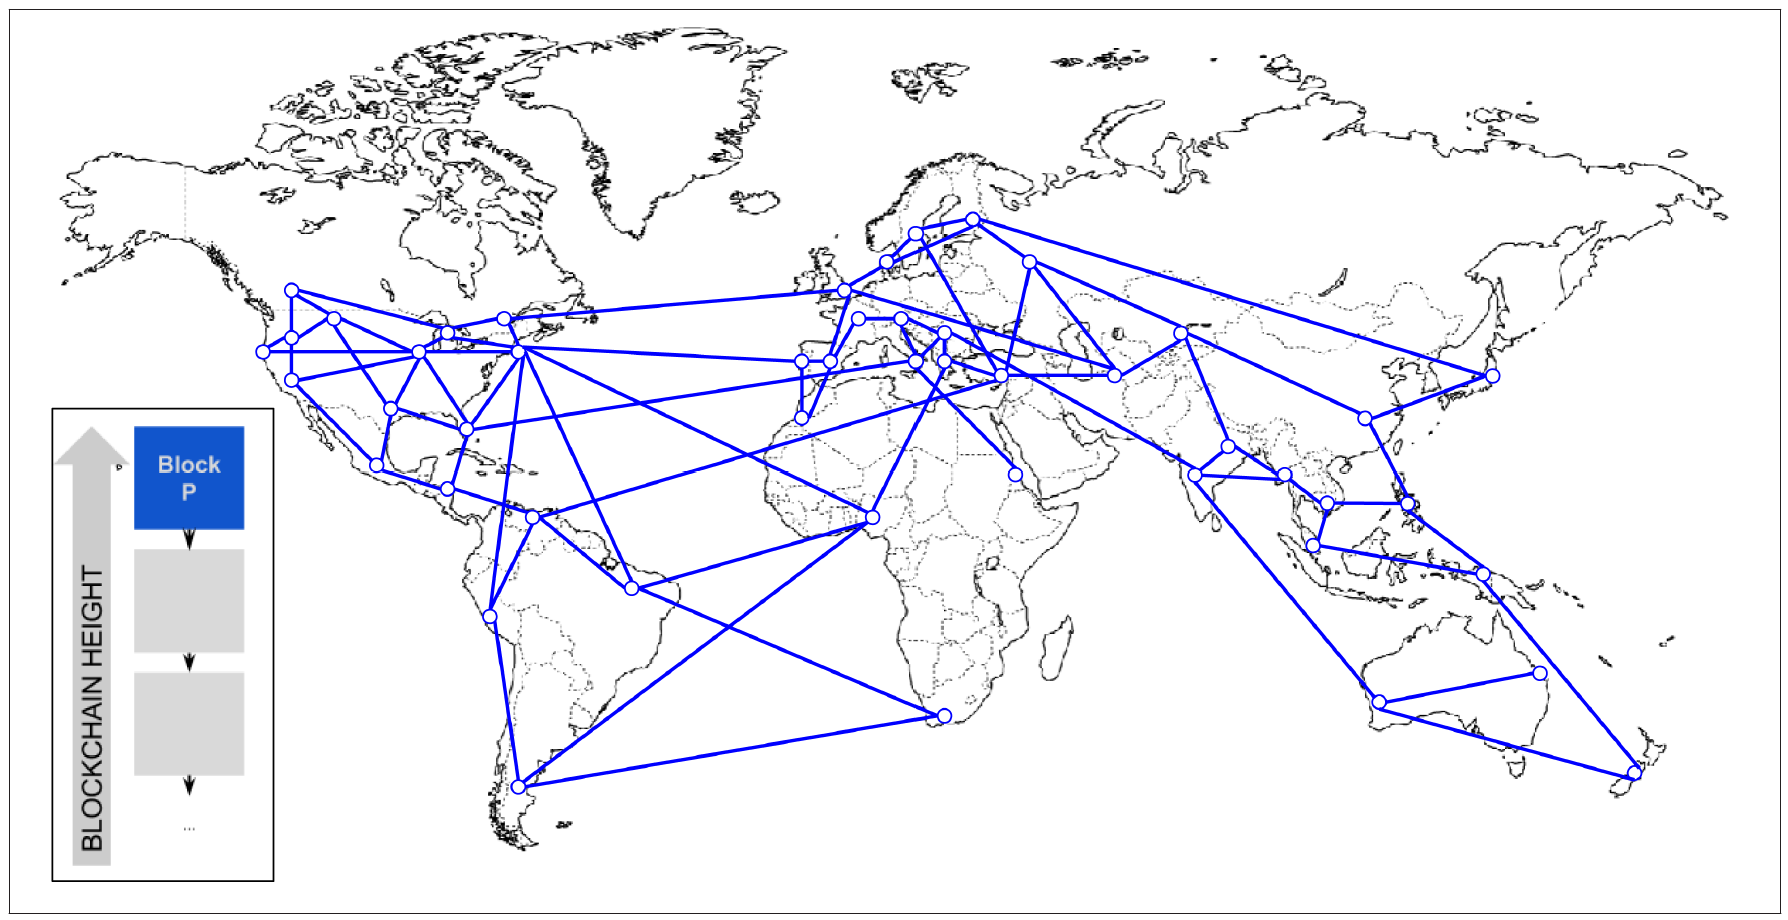
\includegraphics[width=0.85 \linewidth]{figure/fork1}
	\caption{\textit{Visualizzazione di un evento fork--prima della fork} \label{fig:fork1}}
\end{figure}

Un evento \textit{fork} avviene quando ci sono due diversi blocchi che sono candidati ad essere aggiunti contemporaneamente alla Blockchain. Ciò può accadere quando due diversi miner risolvono la proof of work con uno scarto di tempo molto piccolo tra entrambi. Di conseguenza, tali miner immediatamente rivelano la loro soluzione in modo broadcast, e il nuovo blocco creato viene trasmesso tempestivamente ai loro vicini, che propagano i blocchi nuovi attraverso la rete. 

Ogni nodo che riceve un blocco valido, lo incorpora all'interno della propria versione della blockchain, allungandola di un blocco. Se tale nodo si rende conto di aver ricevuto un ulteriore blocco che soddisfa le condizioni, lo aggiunge creando una catena secondaria alternativa al blocco aggiunto appena prima.

In \textit{figura \ref{fig:fork2}} si possono notare due miner che hanno minato due diversi blocchi quasi simultaneamente.\\
Entrambi i blocchi sono figli del blocco blu, ed hanno lo scopo di estendere la chain aggiungendosi sopra al blocco blu. Nella figura, un blocco è rappresentato in rosso e l'altro in verde.
\begin{figure}[h]
	\centering
	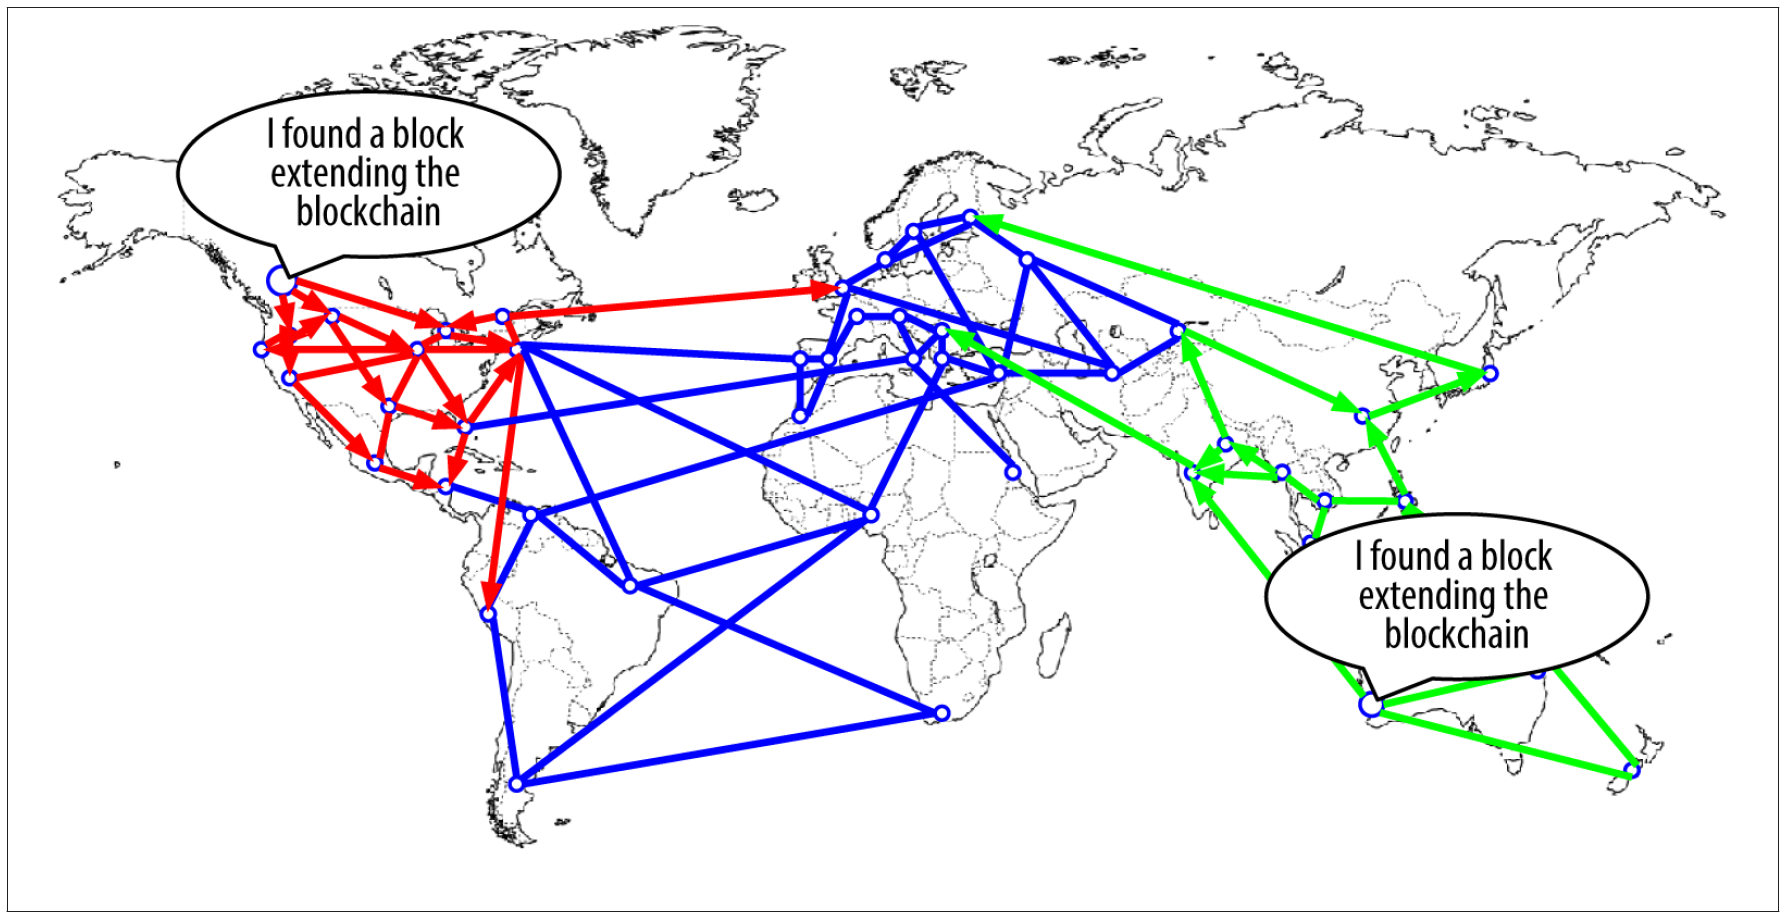
\includegraphics[width=0.85 \linewidth]{figure/fork2}
	\caption{\textit{Visualizzazione di un evento fork: due blocchi minati simultaneamente} \label{fig:fork2}}
\end{figure}
Per esempio, si assuma che un miner in Canada trova una soluzione proof of work per il blocco "rosso" che estende la blockchain come figlio del blocco "blu". Quasi simultaneamente, un altro miner in Australia trova un'altra soluzione per il blocco "verde" al fine di estendere la blockchain. Entrambi i blocchi sono validi, entrambi contengono una soluzione valida alla proof of work, e tutti e due sono figli del blocco "blu". Inoltre, entrambi contengono quasi le stesse transazioni, con solo alcune piccole differenze.

Appena i due blocchi vengono propagati, alcuni nodi ricevono il blocco "rosso" e altri il blocco "verde". Come si può vedere in \textit{figura \ref{fig:fork3}}, la rete si divide in due diverse prospettive della blockchain, un lato con all'estremità il blocco rosso e l'altro lato con il blocco verde.
\begin{figure}[hbp]
	\centering
	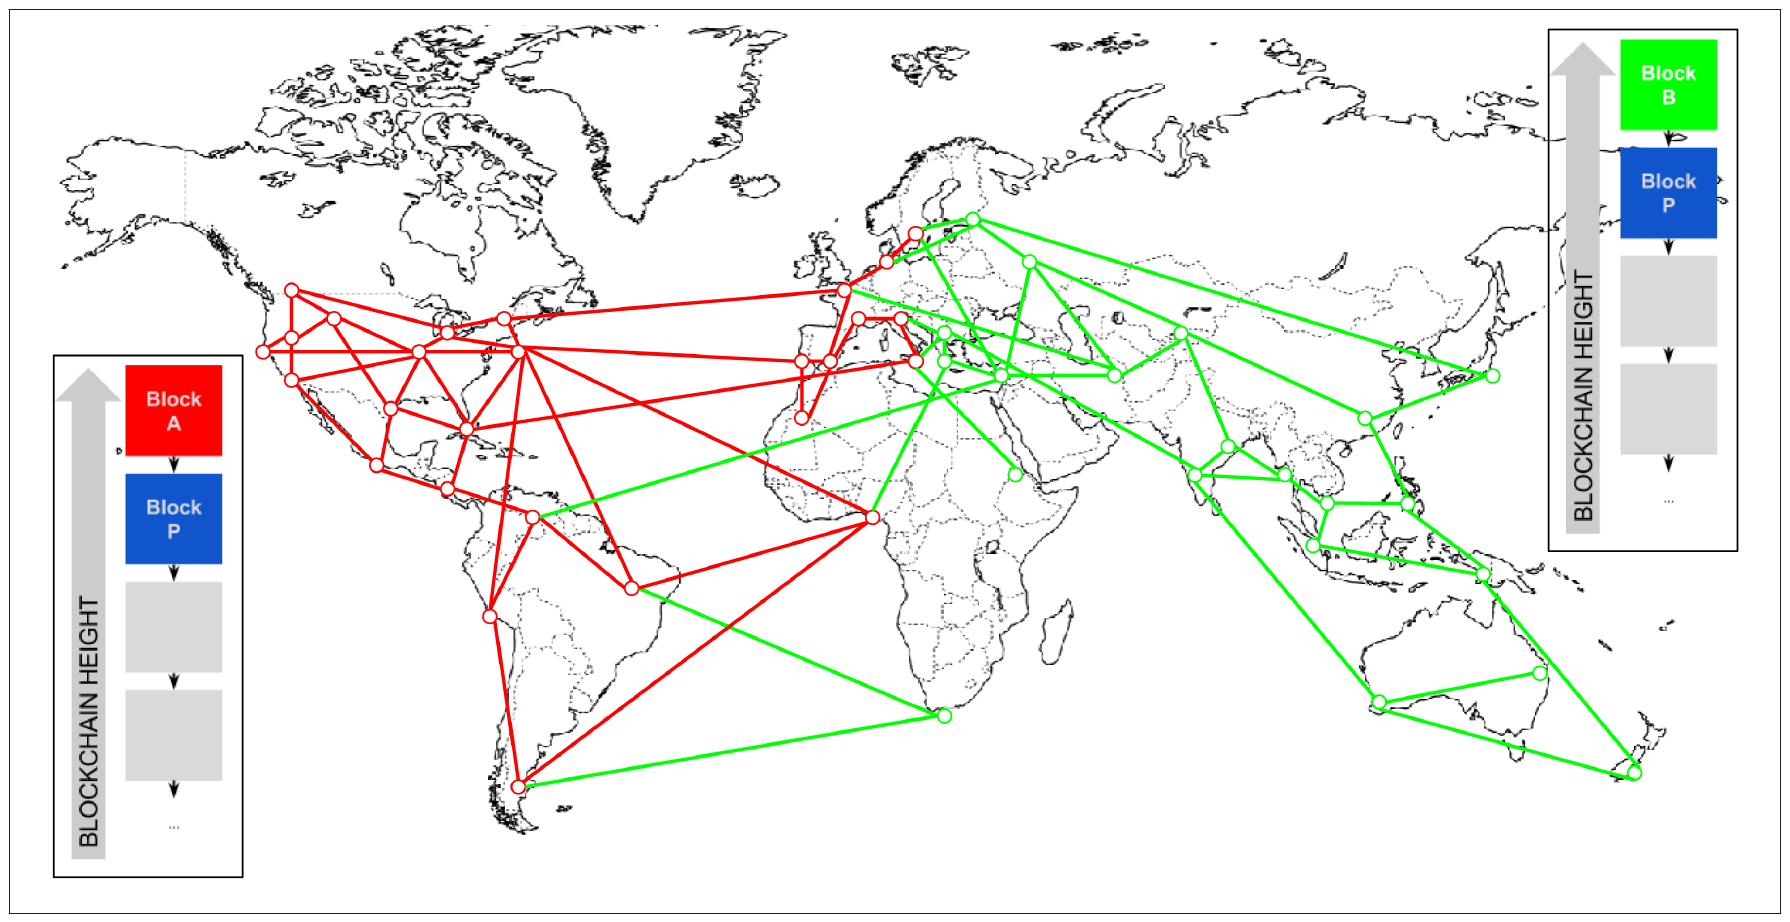
\includegraphics[width=0.85 \linewidth]{figure/fork3}
	\caption{\textit{Visualizzazione di un evento fork: due blocchi propagati, la rete biforca} \label{fig:fork3}}
\end{figure}
Da quel momento, i nodi della rete che sono più vicini al nodo del Canada, aggiungeranno anch'essi il blocco "rosso" per primo, e creeranno una nuova blockchain con il blocco "rosso" come ultimo blocco, ignorando il blocco "verde", che è arrivato un po' più tardi. Nello stesso momento, i nodi più vicini al nodo dell'Australia prenderà il blocco "verde" come vincitore e lo userà per estendere la sua versione della blockchain, aggiungendolo al blocco "blu", ignorando il blocco "rosso" che è arrivato un po' più tardi degli altri. Di conseguenza, ogni miner che vede aggiungere il blocco "rosso" in testa alla chain, immediatamente cercherà di creare altri blocchi che si aggiungeranno al blocco "rosso", ed andrà a risolvere la proof of work per tali blocchi candidati. Invece, i miners che accettano il blocco "verde" cominceranno ad estendere la porzione di chain che si andrà ad attaccare a tale blocco.

Le fork vengono quasi sempre risolte da un singolo blocco. Infatti, come parte del potere computazionale viene dedicato per aggiungere il blocco "rosso", un'altra parte della rete impiega le sue risorse per aggiungere il blocco "verde". Anche se il potere computazionale è quasi diviso in due parti, probabilmente un gruppo di miner troverà e propagherà la soluzione prima che lo faccia un altro gruppo di ulteriori miner. Per esempio, si supponga che i miner trovino un blocco "rosa" che estenda il blocco "verde", immediatamente lo propagherebbero all'intera rete (\textit{figura \ref{fig:fork4}}).

\begin{figure}[hbp]
	\centering
	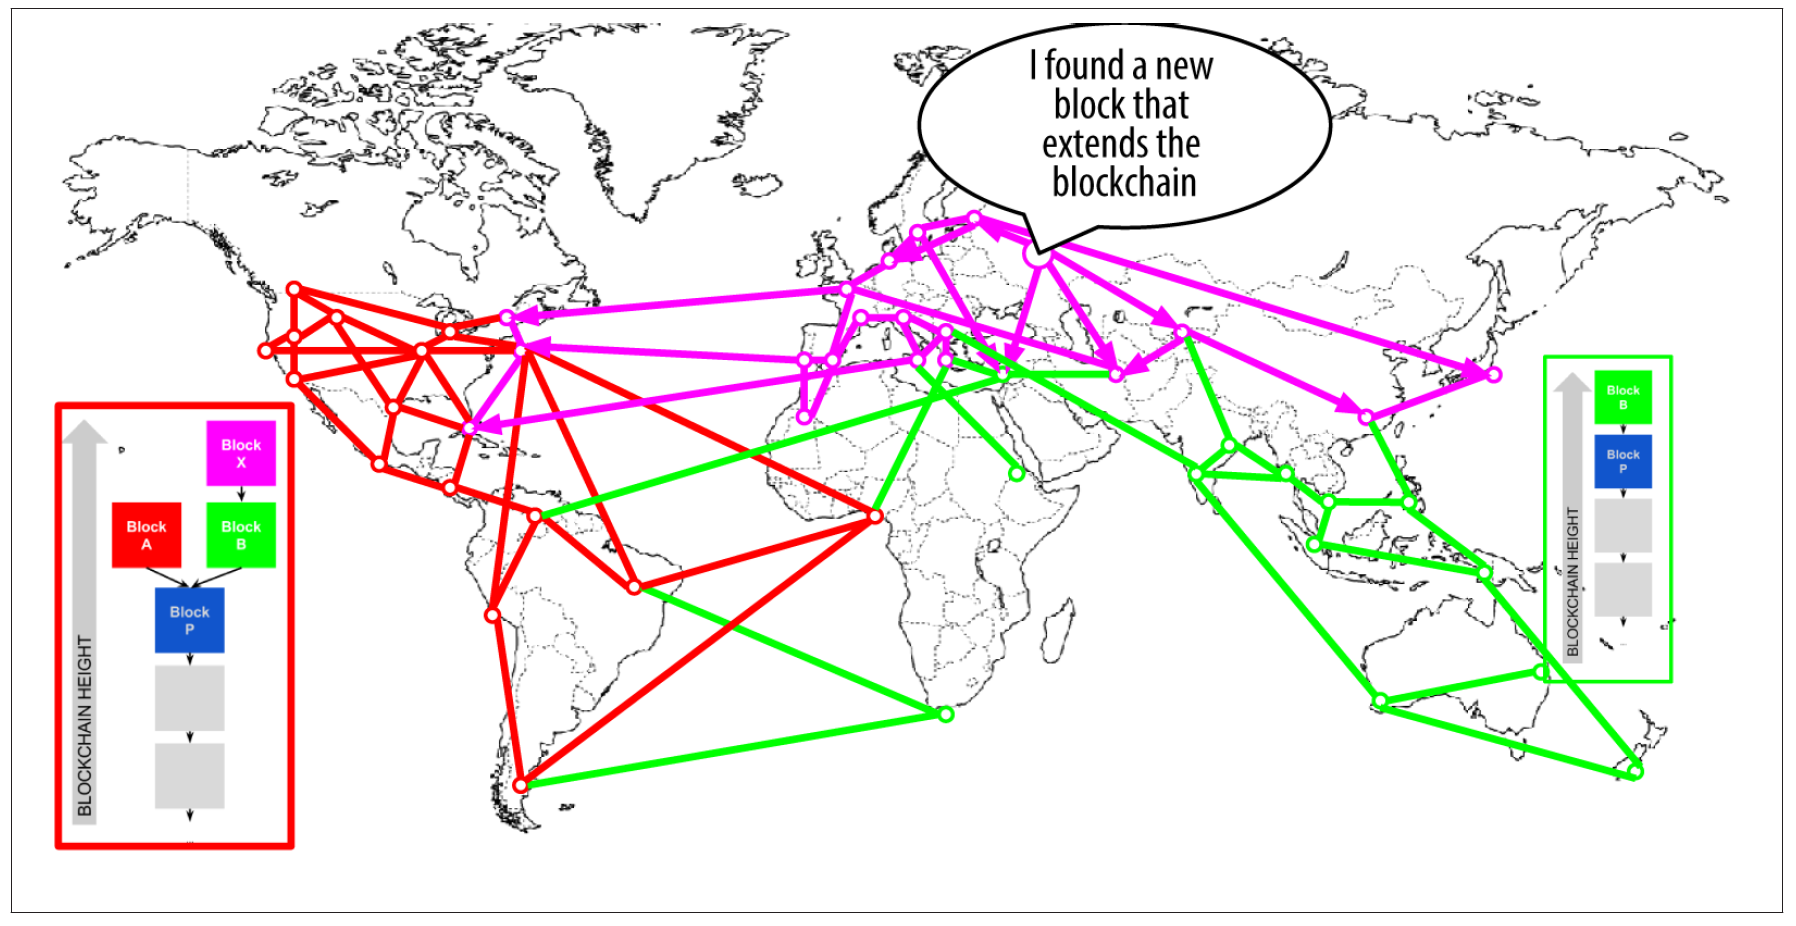
\includegraphics[width=0.85 \linewidth]{figure/fork4}
	\caption{\textit{Visualizzazione di un evento fork: un nuovo blocco estende un ramo della fork} \label{fig:fork4}}
\end{figure}

Tutti i nodi che hanno scelto il blocco "verde" come vincitore nel round precedente, estenderanno la catena di un ulteriore blocco. I nodi che hanno scelto il blocco "rosso" come vincitore, quindi, vedranno due chain: quella blu-verde-rosa e quella blu-rossa. La chain blu-verde-rosa è la più lunga, ovvero è più difficile trovare una prook of work per essa. Inoltre, in \textit{figura \ref{fig:fork5}} si possono vedere i nodi che hanno scelto come catena principale la chain blu-verde-rosa e come chain secondaria quella blu-rossa.
\begin{figure}[hbp]
	\centering
	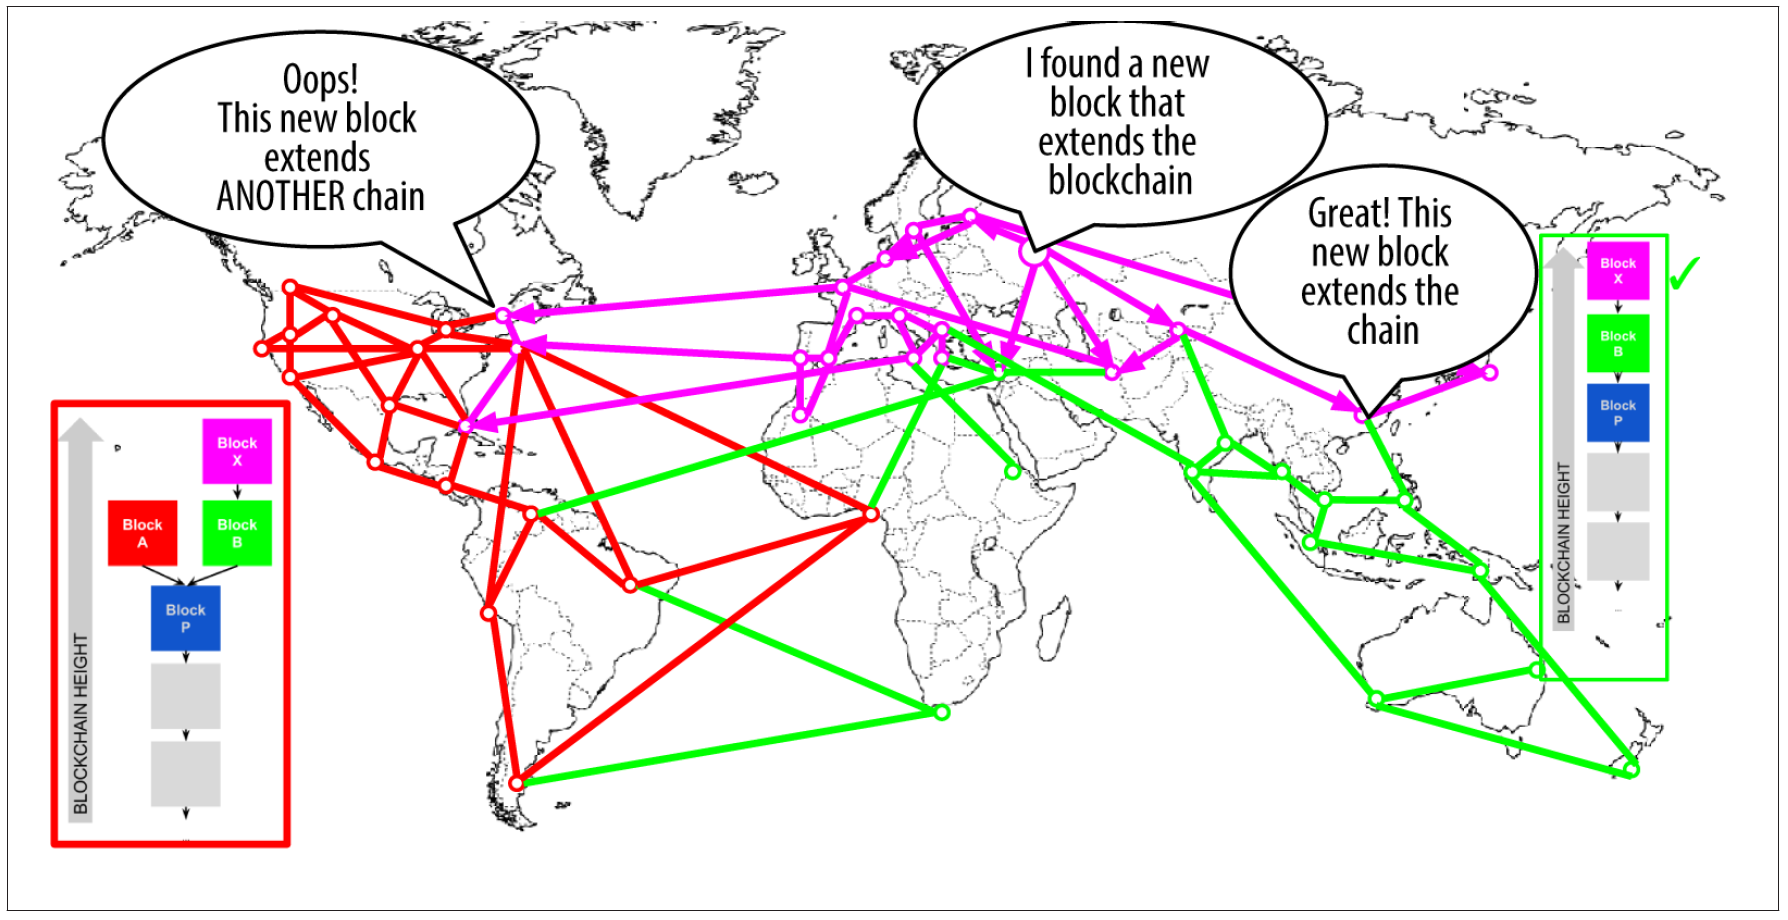
\includegraphics[width=0.85 \linewidth]{figure/fork5}
	\caption{\textit{Visualizzazione di un evento fork: la rete si riunisce in un'unica catena più lunga} \label{fig:fork5}}
\end{figure}

Questo processo è detto \textit{chain reconvergence}(letteralmente riconvergenza della catena), perchè tali nodi vengono forzati a cambiare il loro punto di vista della blockchain al fine di considerare la catena più lunga tra le due.\\ Ogni miner che lavora per estendere la chain blu-rossa non potrà più continuare poichè il blocco che stanno tentando di aggiungere al blocco rosso rimarrà "orfano", dato che il blocco rosso che dovrebbe fare da genitore non appartiene alla chain più lunga della blockchain. \\ Le transazioni che sono all'interno del blocco "rosso", vengono inserite di nuovo in coda per essere processate in un nuovo blocco, perchè, come si è già detto, il blocco a cui appartenevano non fa più parte della blockchain.

L'intera rete, quindi, riconverge la blockchain in una catena singola che fa capo ai blocchi blu-verde-rosa, con il blocco "rosa" come ultimo blocco all'estremità della catena. Tutti i miner immediatamente cominceranno a candidare nuovi blocchi che si andranno ad attaccare al blocco "rosa", al fine di estendere la catena blu-verde-rosa.

Teoricamente potrebbe essere possibile per una fork estendere due blocchi diversi, ma solamente se tali blocchi vengono creati quasi simultaneamente da miner che sono su "lati" diversi di una fork precedente. Tuttavia, la probabilità che ciò accada è molto bassa. Anche se ci fosse una fork ogni settimana, una fork a due blocchi è molto rara.

L'intervallo tra un blocco e il suo successivo è all'incirca di 10 minuti, proprio perché è stato progettato per essere un compromesso tra la velocità dei tempi di ricezione delle conferme e la probabilità di una fork. Un intervallo più ristretto da un lato potrebbe rendere le transazioni più veloci, dall'altro potrebbe causare fork più frequenti. Al contrario, un intervallo più ampio farebbe diminuire il numero delle fork ma renderebbe più lenti i pagamenti.

\section{Le Transazioni}

Come è stato detto in precedenza, una transazione è uno scambio di monete bitcoin tra due o più individui. Per esempio, se Alice vuole dare 1BTC a Bob, ha bisogno di effettuare una transazione inserendo come input l'importo da trasferire e l'indirizzo del wallet di Bob. \\ 

Nella maggior parte dei casi, la quantità di denaro che partecipa alla transazione non è quasi mai
Secondo la configurazione predefinita dal protocollo, quando viene effettuata una transazione che non implica la spesa dell'intero importo contenuto nel wallet del mittente, è previsto che venga creata un ulteriore transazione con il 

Una caratteristica delle transazioni è che possono partecipare più wallet contemporaneamente: ad esempio, un individuo può inviare con la stessa transazione, una quantità di bitcoin a due individui diversi, in modo da recapitare ciascuno la quantità di bitcoin desiderata. 

\section{Grafo delle transazioni}
\section{Caratteristiche del grafo}